%% rnaastex.cls is the classfile used for Research Notes. It is derived
%% from aastex61.cls with a few tweaks to allow for the unique format required.
%% (10/15/17)
%%\documentclass{rnaastex}

%% Better is to use the "RNAAS" style option in AASTeX v6.2
%% (01/08/18)
%\documentclass[RNAAS, a4paper]{aastex631} % RNAAS -- successful compile
\documentclass[RNAAS, a4paper, dvipdfmx]{aastex631} % local compile

\usepackage{xcolor}
%% Define new commands here
%\newcommand\latex{La\TeX}
\newcommand\fobl{f_{\rm obl}}
\newcommand\wR{\omega_{\rm R}}
\newcommand\wDR{\omega_{\rm DR}}
\newcommand\wHSCF{\omega_0}

\begin{document}

\title{Fitting rotational frequency of polytropes as a function of their oblateness (unsubmitted version)}

%% Note that the corresponding author command and emails has to come
%% before everything else. Also place all the emails in the \email
%% command instead of using multiple \email calls.
\author{Shin'ichirou Yoshida}
\email{yoshida@ea.c.u-tokyo.ac.jp}
\affiliation{Department of Earth Science and Astronomy, Graduate School of Arts and Sciences,
The University of Tokyo\\
3-8-1 Komaba, Meguro-ku, Tokyo 153-18902, Japan}


%% Note that RNAAS manuscripts DO NOT have abstracts.
%% See the online documentation for the full list of available subject
%% keywords and the rules for their use.

\begin{abstract}
\textcolor{red}{(This preliminary version for RNAAS submission fits all the polytropic data ($1\le N\le 3$)
with a single Pad\'{e} formula, as well as a single polynomial.)}\\
Giving a simple functional relation between the rotational frequency and
the deformation for compressible stellar models is useful both in observational
and theoretical astrophysics.
Here I present simple formulae for the rotational frequency of polytropic
stars as a function of the oblateness, which is valid for a different polytropic
index in $1\le N\le 3$ and the speed of rotation up to the mass-shedding limit.
\end{abstract}

\keywords{Stellar rotation}

%% Start the main body of the article. If no sections in the 
%% research note leave the \section call blank to make the title.
\section{} 

In \cite{Yoshida}, I presented assessment of the Roche
and the Darwin-Radau approximation which are often used in studying
rotating stars. Here I report a simple formula of a dimensionless stellar
angular frequency $\omega$ as a function of its oblateness, which
is derived by fitting numerical hydrostatic equilibria for a range of
polytropic equation of state (EOS).


The equilibrium models are computed by a numerical code for 
rotating hydrostatic two-dimensional equilibria.
The code is written by the author and tested against the existing
results \citep{HSCF}. The code self-consistently takes into account
the inhomogeneous gas distribution and its self-gravity. The assumption
of slow-rotation is not necessary and the models up to the mass-shedding
limit are obtained.

I focus on the property of rotating polytropes whose EOS is
\begin{equation}
	p = K \rho^{1+\frac{1}{N}},
\end{equation}
where $p$ and $\rho$ are the pressure and the density. $K$ is a constant
and $N$ is a constant called polytropic index. 

Given $N$, the rotational angular frequency $\omega$ normalized by the factor $\sqrt{GM/R_e^3}$
is fitted, where $M$ is the mass and $R_e$ is the equatorial radius. As for the independent
parameter, the normalized oblateness, $f_{\rm obl}/f_{\rm obl, MS}\equiv\tilde{f}_o$, is chosen,
where $f_{\rm obl} = 1-R_p/R_e$ and $R_p$ is the polar radius or the object.
Notice that $0\le \tilde{f}_o \le 1$.
$f_{\rm obl, MS}$ is the oblateness at the mass-shedding limit for the $N$ value.
The oblateness at the mass-shedding limit depends on the EOS. Thus I also
make a fitting formula of $f_{\rm obs, MS} (\Gamma)$, where $\Gamma = 1+1/N$.

Assumed functional form of the fitting formula of $\omega^2$ is the Pad\`{e} form,
\begin{equation}
	\omega^2(\tilde{f}_o) = \frac{\tilde{f}_o (a_0 + a_1 \tilde{f}_o)}{1 + a_2 \tilde{f}_o}
	\label{eq:omega2}
\end{equation}
and that of $f_{\rm obl, MS}$ as,
\begin{equation}
	f_{\rm obl, MS}(\Gamma) = \frac{b_0 + b_1 \Gamma}{1 + b_2 \Gamma}
	\label{eq:foblMS}
\end{equation}

I use the nonlinear least square fitting module of {\tt scipy.optimize.curve\_fit}
to fit the numerical data.
\footnote{\url{https://docs.scipy.org/doc/scipy/reference/generated/scipy.optimize.curve_fit.html}
}
For the fitting of Eq.(\ref{eq:omega2}), I compute 694
models of polytropes with $N=(1.0, 1.1, 1.2, 1.4, 1.5, 1.6, 1.8, 2.0, 2.2, 2.5, 3.0)$
from non-rotating to maximally rotating (mass-shedding) cases.

The left panel of Fig.\ref{fig:1} shows the fitting of the $\omega^2$ data with an analytic 
form. All the data of different $N$ is weighted equally in the fitting. It is seen that the
simple form of Eq.(\ref{eq:omega2}) approximates the numerical data
within a few percent of errors, though the error increases steeply
as the model approaches the mass-shedding limit.
The right panel of Fig.\ref{fig:1} is $f_{\rm MS}$ and its fitting curve.


The fitting parameters obtained for $\omega^2$ are,
\begin{equation}
	a_0 = 0.6042, ~a_1=-0.07372, ~a_2=-0.4891, 
\end{equation}
and for $f_{\rm MS}$ are,
\begin{equation}
	b_0=0.1820,~ b_1=0.05912,~ b_2=-0.1619.
\end{equation}

%% An example figure call using \includegraphics
\begin{figure}[h!]
\begin{center}
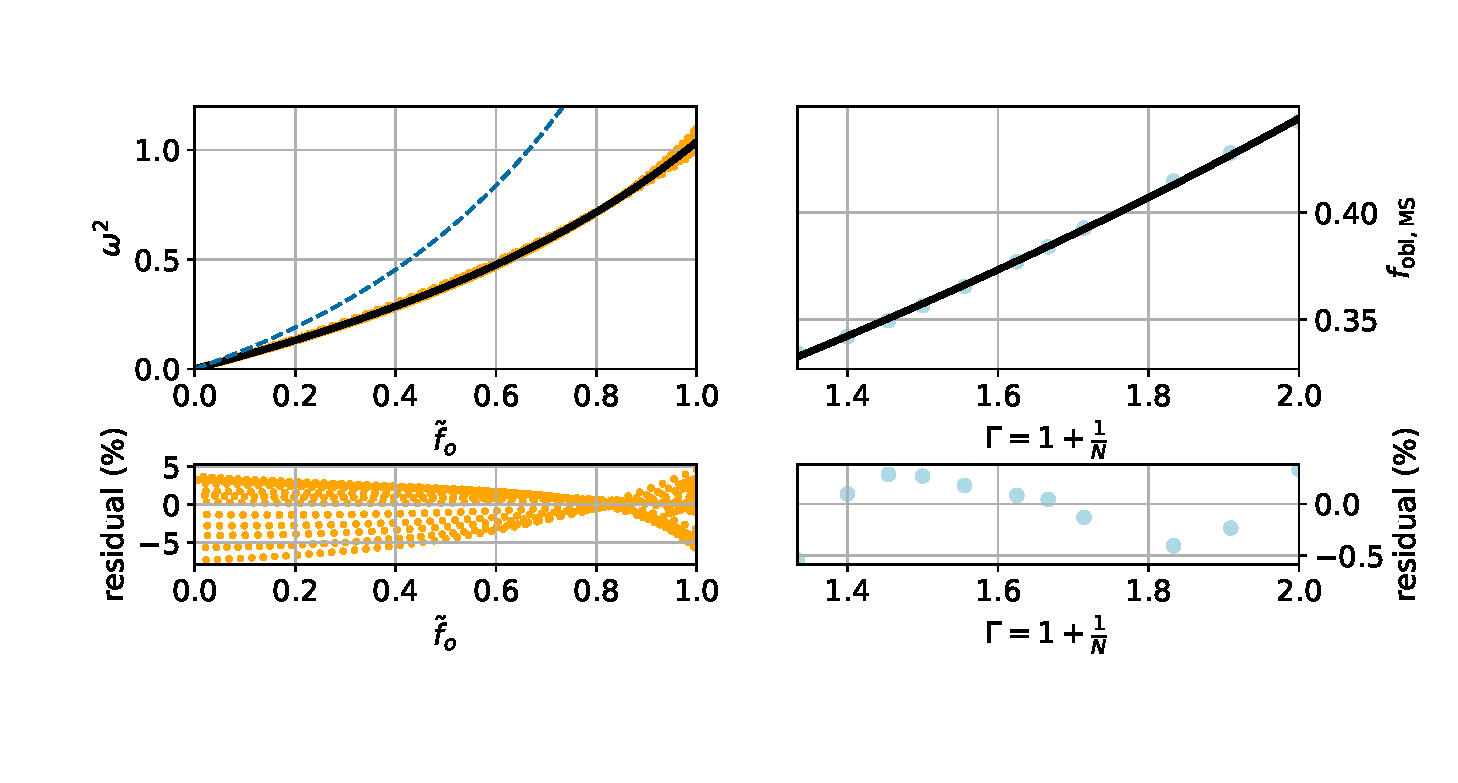
\includegraphics[scale=0.7]{fittingW2.eps}
\caption{Left: Normalized $\omega^2$ versus normalized oblateness$\tilde{f_o}$. Orange points
are numerical data and the solid black line is the fitted formula by Eq.(\ref{eq:omega2}).
The dashed line is the curve for the incompressible Maclaurin spheroid \citep{Chandrasekhar}
in our normalization  (for which $f_{\rm obl, MS}=1$) .
The bottom panel shows the relative residuals (in percent) of the fitting. Notice that the
large residual for $\tilde{f}_o\to 0$ is an artifact of the behavior of $\omega^2\to 0$. 
Right: The oblateness at the mass-shedding limit
versus the adiabatic index $\Gamma$. The light blue points are numerical data, while
the solid black line is the fitted formula by Eq.(\ref{eq:foblMS}).
The bottom panel shows the residuals.
\label{fig:1}}
\end{center}
\end{figure}
%%%%%%

Alternatively, if a simple polynomial form,
\begin{equation}
	\omega^2 = \tilde{f}_0\sum_{j=0}p_j \tilde{f}_o^j,
\end{equation}
is chosen, a fitting with the minimal number of terms 
is done in a similar size of the error with,
\begin{equation}
	p_0=0.6020,~ p_1=0.2655,~ p_2=-0.04464,~ p_3=0.2148.
\end{equation}

%\acknowledgments

\begin{thebibliography}{}

\bibitem[Chandrasekhar(1987)]{Chandrasekhar} Chandrasekhar, S., \ 1987, Ellipsoidal Figures of Equilibrium, Dover, New York

\bibitem[Hachisu(1986)]{HSCF} Hachisu, I., \ 1986, \apjs, {\bf 61}, 479

\bibitem[Yoshida (2022)]{Yoshida} Yoshida, S., \ 2022, RNAAS, in press

\end{thebibliography}

\end{document}
